\documentclass{article}\usepackage[]{graphicx}\usepackage[]{color}
%% maxwidth is the original width if it is less than linewidth
%% otherwise use linewidth (to make sure the graphics do not exceed the margin)
\makeatletter
\def\maxwidth{ %
  \ifdim\Gin@nat@width>\linewidth
    \linewidth
  \else
    \Gin@nat@width
  \fi
}
\makeatother

\definecolor{fgcolor}{rgb}{0.345, 0.345, 0.345}
\newcommand{\hlnum}[1]{\textcolor[rgb]{0.686,0.059,0.569}{#1}}%
\newcommand{\hlstr}[1]{\textcolor[rgb]{0.192,0.494,0.8}{#1}}%
\newcommand{\hlcom}[1]{\textcolor[rgb]{0.678,0.584,0.686}{\textit{#1}}}%
\newcommand{\hlopt}[1]{\textcolor[rgb]{0,0,0}{#1}}%
\newcommand{\hlstd}[1]{\textcolor[rgb]{0.345,0.345,0.345}{#1}}%
\newcommand{\hlkwa}[1]{\textcolor[rgb]{0.161,0.373,0.58}{\textbf{#1}}}%
\newcommand{\hlkwb}[1]{\textcolor[rgb]{0.69,0.353,0.396}{#1}}%
\newcommand{\hlkwc}[1]{\textcolor[rgb]{0.333,0.667,0.333}{#1}}%
\newcommand{\hlkwd}[1]{\textcolor[rgb]{0.737,0.353,0.396}{\textbf{#1}}}%

\usepackage{framed}
\makeatletter
\newenvironment{kframe}{%
 \def\at@end@of@kframe{}%
 \ifinner\ifhmode%
  \def\at@end@of@kframe{\end{minipage}}%
  \begin{minipage}{\columnwidth}%
 \fi\fi%
 \def\FrameCommand##1{\hskip\@totalleftmargin \hskip-\fboxsep
 \colorbox{shadecolor}{##1}\hskip-\fboxsep
     % There is no \\@totalrightmargin, so:
     \hskip-\linewidth \hskip-\@totalleftmargin \hskip\columnwidth}%
 \MakeFramed {\advance\hsize-\width
   \@totalleftmargin\z@ \linewidth\hsize
   \@setminipage}}%
 {\par\unskip\endMakeFramed%
 \at@end@of@kframe}
\makeatother

\definecolor{shadecolor}{rgb}{.97, .97, .97}
\definecolor{messagecolor}{rgb}{0, 0, 0}
\definecolor{warningcolor}{rgb}{1, 0, 1}
\definecolor{errorcolor}{rgb}{1, 0, 0}
\newenvironment{knitrout}{}{} % an empty environment to be redefined in TeX

\usepackage{alltt}
\IfFileExists{upquote.sty}{\usepackage{upquote}}{}
\begin{document}

\begin{knitrout}
\definecolor{shadecolor}{rgb}{0.969, 0.969, 0.969}\color{fgcolor}\begin{kframe}
\begin{alltt}
\hlcom{#GUIA 9}
\hlkwd{ls}\hlstd{()}
\end{alltt}
\begin{verbatim}
## character(0)
\end{verbatim}
\begin{alltt}
\hlkwd{rm}\hlstd{(}\hlkwc{list}\hlstd{=}\hlkwd{ls}\hlstd{(}\hlkwc{all}\hlstd{=}\hlnum{TRUE}\hlstd{))}
\hlkwd{ls}\hlstd{()}
\end{alltt}
\begin{verbatim}
## character(0)
\end{verbatim}
\begin{alltt}
\hlkwd{library}\hlstd{(foreign)}
\end{alltt}


{\ttfamily\noindent\color{warningcolor}{\#\# Warning: package 'foreign' was built under R version 3.2.2}}\begin{alltt}
\hlstd{HojaCat} \hlkwb{<-} \hlkwd{read.csv}\hlstd{(}\hlstr{"HojaCat.csv"}\hlstd{,} \hlkwc{strip.white}\hlstd{=}\hlnum{TRUE}\hlstd{);HojaCat}
\end{alltt}
\begin{verbatim}
##        Estado  Ocupacion
## 1      Casado Desocupado
## 2     Soltero    Estudia
## 3     Soltero    Trabaja
## 4      Casado    Estudia
## 5  Acompa�ado    Trabaja
## 6     Soltero Desocupado
## 7      Casado    Trabaja
## 8      Casado    Estudia
## 9  Acompa�ado Desocupado
## 10 Acompa�ado    Estudia
## 11     Casado    Trabaja
## 12    Soltero    Estudia
## 13 Acompa�ado Desocupado
## 14     Casado Desocupado
## 15    Soltero    Estudia
## 16    Soltero    Trabaja
## 17     Casado Desocupado
## 18    Soltero    Trabaja
\end{verbatim}
\begin{alltt}
\hlkwd{attach}\hlstd{(HojaCat,} \hlkwc{pos}\hlstd{=}\hlnum{2}\hlstd{)}
\hlkwd{search}\hlstd{()}
\end{alltt}
\begin{verbatim}
##  [1] ".GlobalEnv"        "HojaCat"           "package:foreign"  
##  [4] "package:knitr"     "package:stats"     "package:graphics" 
##  [7] "package:grDevices" "package:utils"     "package:datasets" 
## [10] "package:methods"   "Autoloads"         "package:base"
\end{verbatim}
\begin{alltt}
\hlstd{tablaCont} \hlkwb{<-} \hlkwd{table}\hlstd{(HojaCat); tablaCont}
\end{alltt}
\begin{verbatim}
##             Ocupacion
## Estado       Desocupado Estudia Trabaja
##   Acompa�ado          2       1       1
##   Casado              3       2       2
##   Soltero             1       3       3
\end{verbatim}
\begin{alltt}
\hlkwd{length}\hlstd{(HojaCat)}
\end{alltt}
\begin{verbatim}
## [1] 2
\end{verbatim}
\begin{alltt}
\hlstd{suma.filas} \hlkwb{<-} \hlkwd{apply}\hlstd{(tablaCont,} \hlnum{1}\hlstd{, sum); suma.filas}
\end{alltt}
\begin{verbatim}
## Acompa�ado     Casado    Soltero 
##          4          7          7
\end{verbatim}
\begin{alltt}
\hlcom{# El 1 indica que son totales por fila}
\hlstd{suma.columnas} \hlkwb{<-} \hlkwd{apply}\hlstd{(tablaCont,}\hlnum{2}\hlstd{,sum); suma.columnas}
\end{alltt}
\begin{verbatim}
## Desocupado    Estudia    Trabaja 
##          6          6          6
\end{verbatim}
\begin{alltt}
\hlcom{# Gr�ficos de barras para tabla de contingencia.}
\hlkwd{barplot}\hlstd{(}\hlkwd{t}\hlstd{(tablaCont),} \hlkwc{main}\hlstd{=}\hlstr{"Grafico de barras (Estado, Ocupacion)"}\hlstd{,} \hlkwc{xlab}\hlstd{=}\hlstr{"Estado civil"}\hlstd{,} \hlkwc{ylab}\hlstd{=}\hlstr{"Ocupacio"}\hlstd{,} \hlkwc{legend.text}\hlstd{=}\hlnum{TRUE}\hlstd{)}
\end{alltt}
\end{kframe}
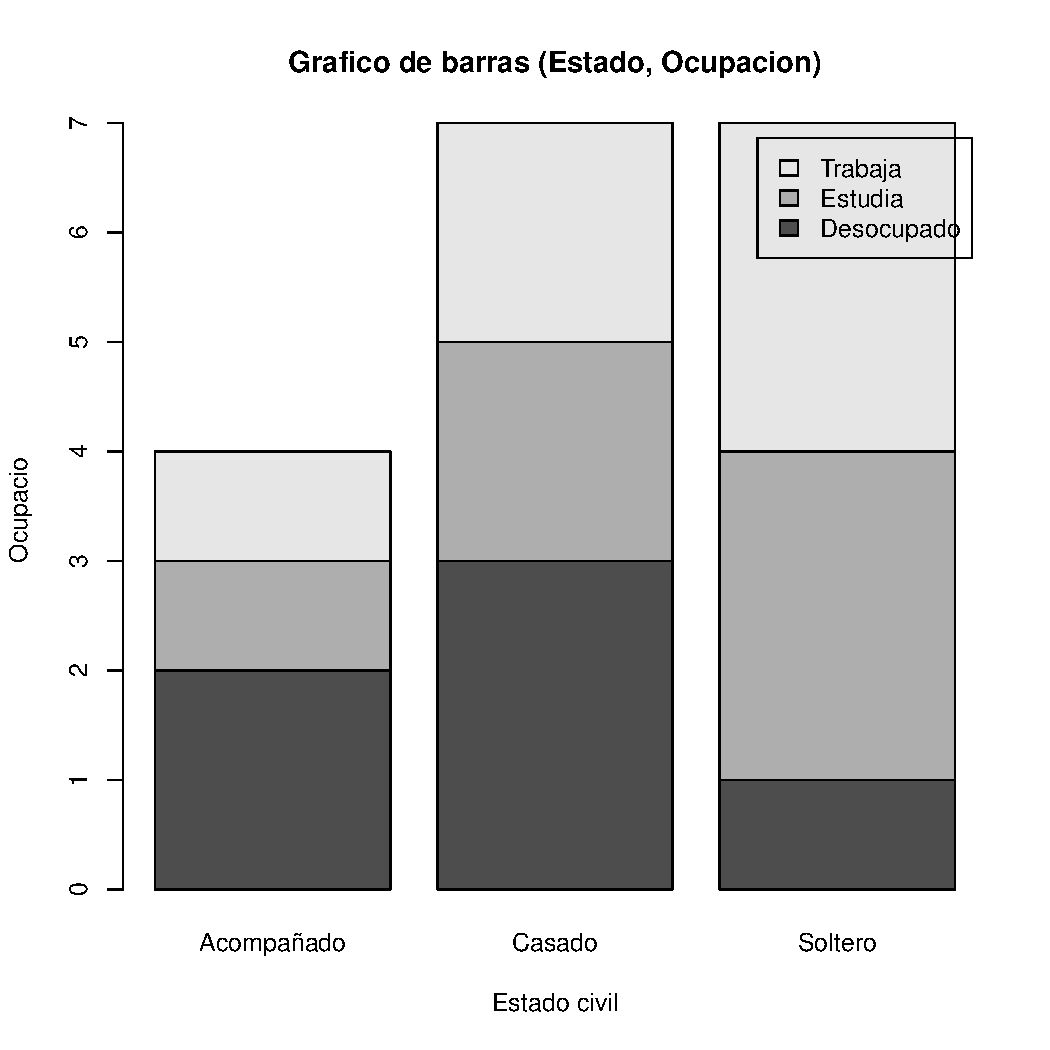
\includegraphics[width=\maxwidth]{figure/unnamed-chunk-1-1} 
\begin{kframe}\begin{alltt}
\hlcom{# Barras agrupadas}
\hlkwd{barplot}\hlstd{(}\hlkwd{t}\hlstd{(tablaCont),} \hlkwc{main}\hlstd{=}\hlstr{"Grafico de barras (Estado, Ocupacion)"}\hlstd{,} \hlkwc{xlab}\hlstd{=}\hlstr{"Estado civil"}\hlstd{,} \hlkwc{ylab}\hlstd{=}\hlstr{"Ocupacion"}\hlstd{,} \hlkwc{beside}\hlstd{=}\hlnum{TRUE}\hlstd{,} \hlkwc{legend.text}\hlstd{=}\hlnum{TRUE}\hlstd{)}
\end{alltt}
\end{kframe}
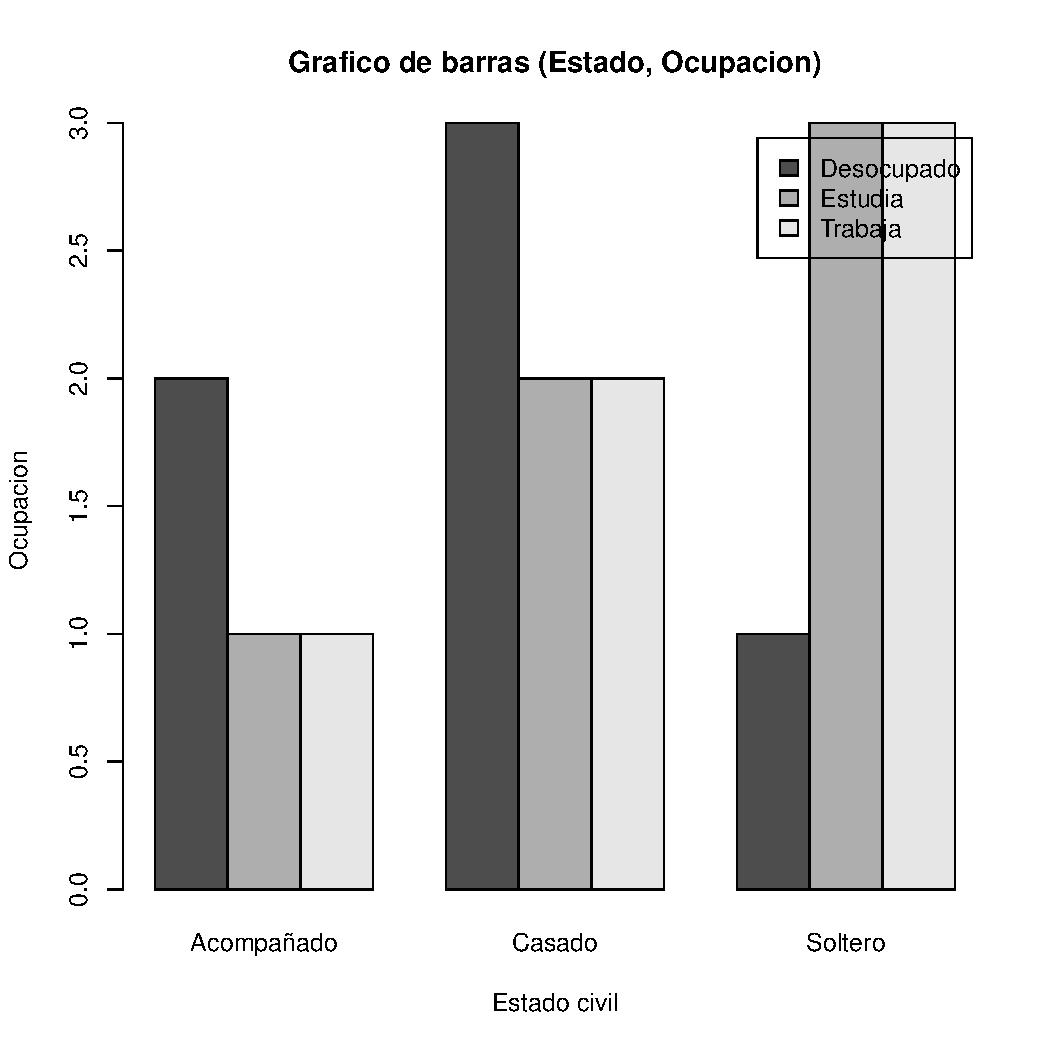
\includegraphics[width=\maxwidth]{figure/unnamed-chunk-1-2} 
\begin{kframe}\begin{alltt}
\hlkwd{barplot}\hlstd{(tablaCont,} \hlkwc{main}\hlstd{=}\hlstr{"Gr�fico de barras (Ocupaci�n, Estado)"}\hlstd{,} \hlkwc{xlab}\hlstd{=}\hlstr{"Ocupaci�n\textbackslash{}n"}\hlstd{,}\hlkwc{ylab}\hlstd{=}\hlstr{"Estado civil"}\hlstd{,} \hlkwc{beside}\hlstd{=}\hlnum{TRUE}\hlstd{,} \hlkwc{legend.text}\hlstd{=}\hlnum{TRUE}\hlstd{)}
\end{alltt}
\end{kframe}
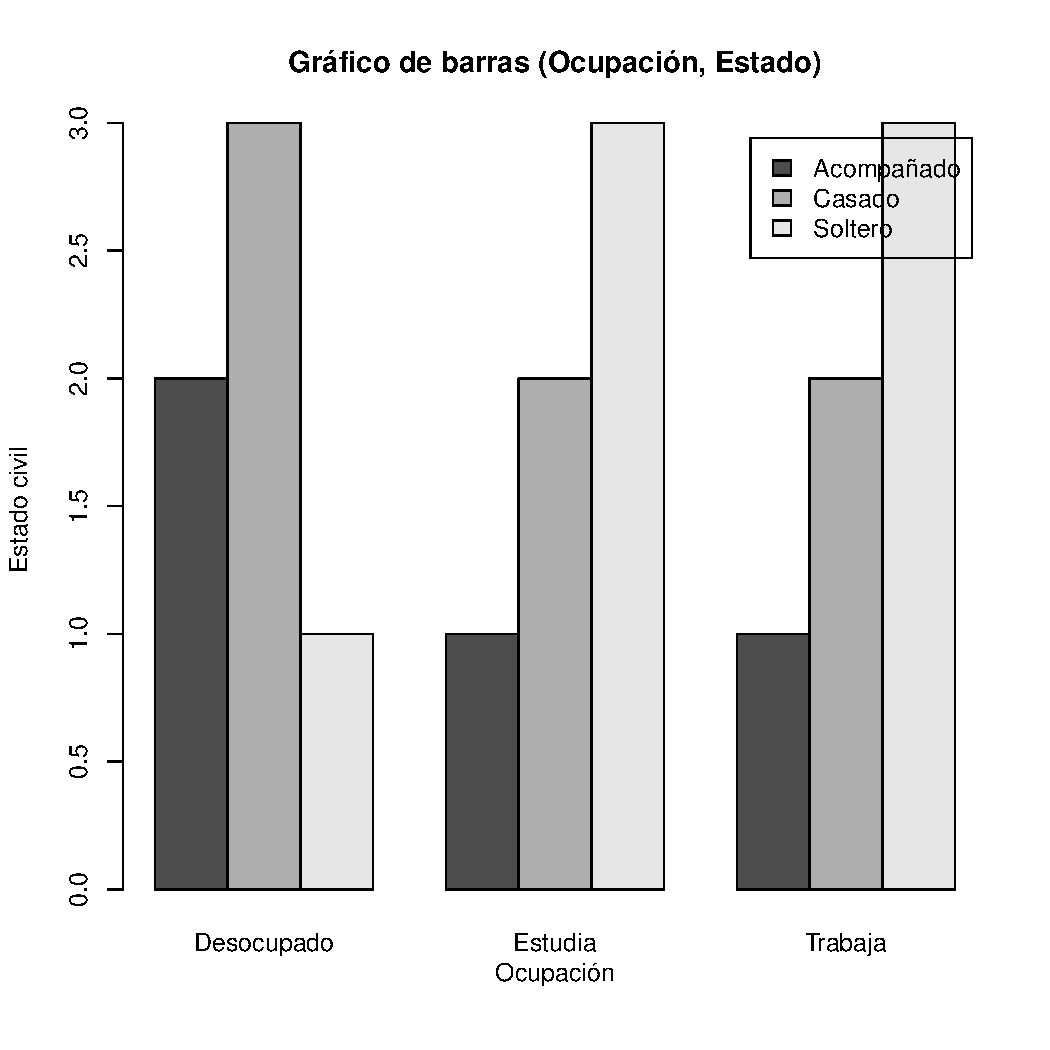
\includegraphics[width=\maxwidth]{figure/unnamed-chunk-1-3} 
\begin{kframe}\begin{alltt}
\hlstd{op} \hlkwb{<-} \hlkwd{options}\hlstd{()}
\hlkwd{options}\hlstd{(}\hlkwc{digits}\hlstd{=}\hlnum{3}\hlstd{)}
\hlkwd{options}\hlstd{(}\hlstr{'digits'}\hlstd{)}
\end{alltt}
\begin{verbatim}
## $digits
## [1] 3
\end{verbatim}
\begin{alltt}
\hlcom{# Proporciones basadas en el total de la muestra, la suma de filas y columnas suman 1}
\hlstd{propTotal} \hlkwb{<-} \hlkwd{prop.table}\hlstd{(tablaCont); propTotal}
\end{alltt}
\begin{verbatim}
##             Ocupacion
## Estado       Desocupado Estudia Trabaja
##   Acompa�ado     0.1111  0.0556  0.0556
##   Casado         0.1667  0.1111  0.1111
##   Soltero        0.0556  0.1667  0.1667
\end{verbatim}
\begin{alltt}
\hlkwd{barplot}\hlstd{(}\hlkwd{t}\hlstd{(propTotal),} \hlkwc{main}\hlstd{=}\hlstr{"Grafico de barras (Estado, Ocupacion)"}\hlstd{,} \hlkwc{xlab}\hlstd{=}\hlstr{"Estado civil\textbackslash{}n"}\hlstd{,}\hlkwc{ylab}\hlstd{=}\hlstr{"Ocupacion"}\hlstd{,} \hlkwc{beside}\hlstd{=}\hlnum{TRUE}\hlstd{,} \hlkwc{legend.text}\hlstd{=}\hlnum{TRUE}\hlstd{)}
\end{alltt}
\end{kframe}
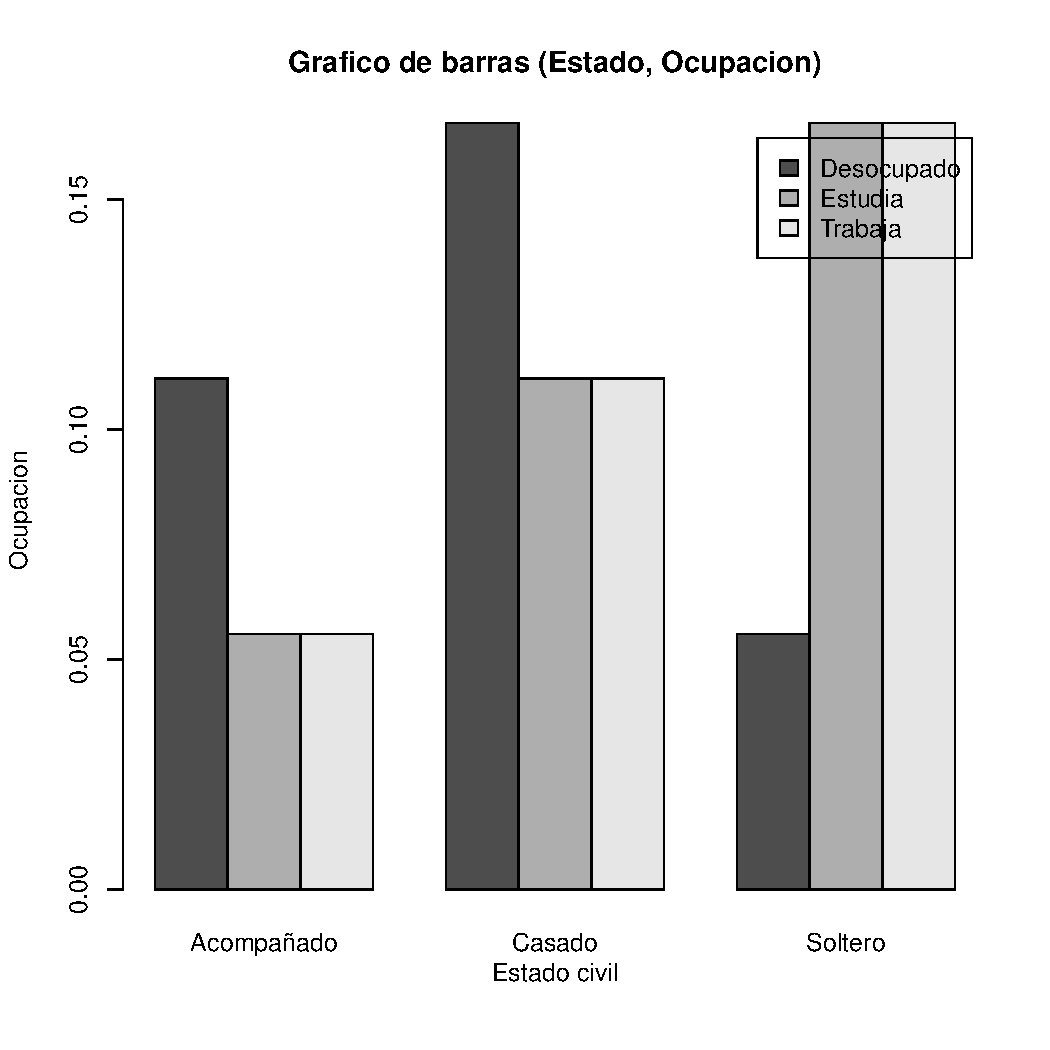
\includegraphics[width=\maxwidth]{figure/unnamed-chunk-1-4} 
\begin{kframe}\begin{alltt}
\hlcom{# Proporciones basadas en el total por fila, cada fila suma 1.}
\hlstd{propFila} \hlkwb{<-} \hlkwd{prop.table}\hlstd{(tablaCont,} \hlnum{1}\hlstd{); propFila}
\end{alltt}
\begin{verbatim}
##             Ocupacion
## Estado       Desocupado Estudia Trabaja
##   Acompa�ado      0.500   0.250   0.250
##   Casado          0.429   0.286   0.286
##   Soltero         0.143   0.429   0.429
\end{verbatim}
\begin{alltt}
\hlcom{# Total por fila se indica en 1}
\hlkwd{barplot}\hlstd{(}\hlkwd{t}\hlstd{(propFila),} \hlkwc{main}\hlstd{=}\hlstr{"Grafico de barras (Estado, Ocupacion)"}\hlstd{,} \hlkwc{xlab}\hlstd{=}\hlstr{"Estado civil\textbackslash{}n"}\hlstd{,}\hlkwc{ylab}\hlstd{=}\hlstr{"Ocupacion"}\hlstd{,} \hlkwc{beside}\hlstd{=}\hlnum{TRUE}\hlstd{,} \hlkwc{legend.text}\hlstd{=}\hlnum{TRUE}\hlstd{)}
\end{alltt}
\end{kframe}
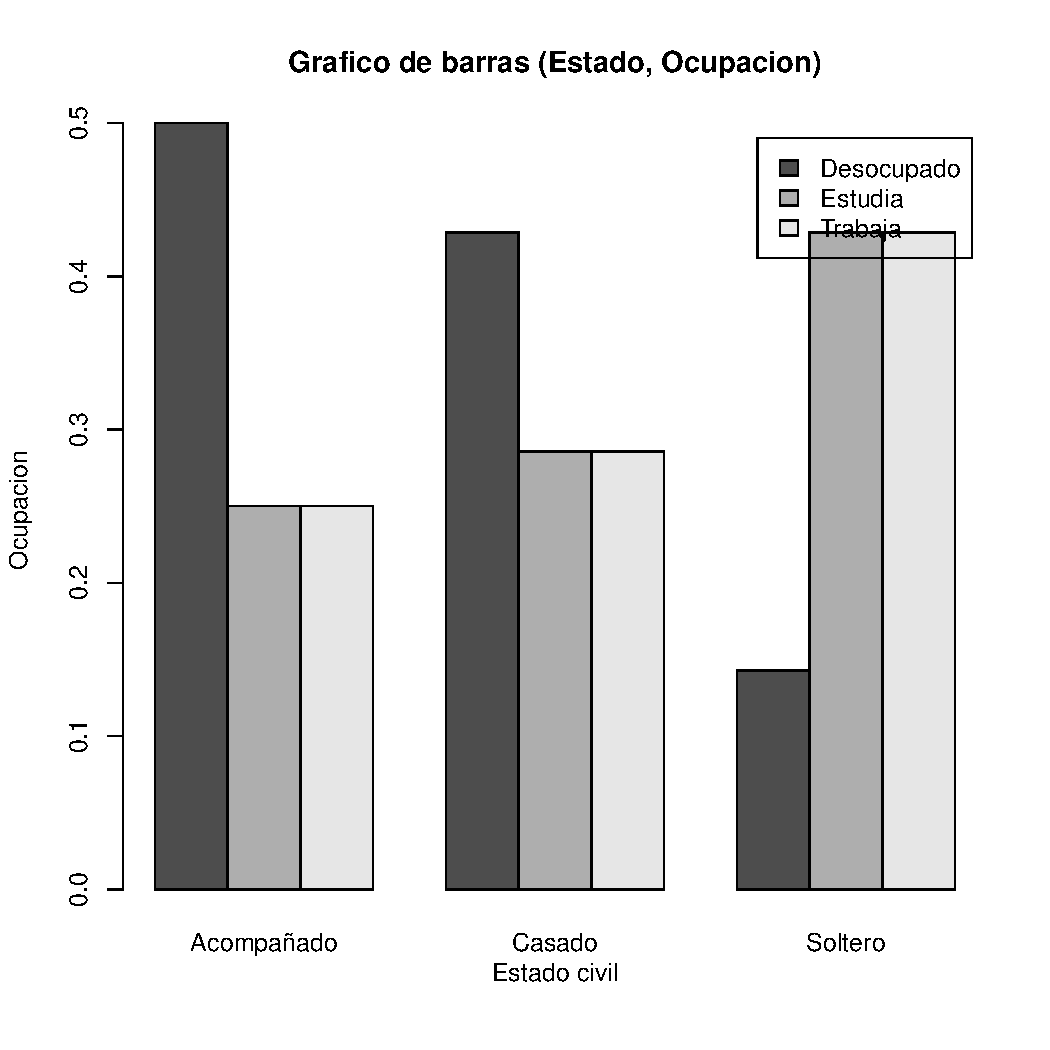
\includegraphics[width=\maxwidth]{figure/unnamed-chunk-1-5} 
\begin{kframe}\begin{alltt}
\hlcom{# Proporciones basadas en el total por columna, cada columna suma 1.}
\hlstd{propColum} \hlkwb{<-} \hlkwd{prop.table}\hlstd{(tablaCont,} \hlnum{2}\hlstd{); propColum}
\end{alltt}
\begin{verbatim}
##             Ocupacion
## Estado       Desocupado Estudia Trabaja
##   Acompa�ado      0.333   0.167   0.167
##   Casado          0.500   0.333   0.333
##   Soltero         0.167   0.500   0.500
\end{verbatim}
\begin{alltt}
\hlcom{# Total por columna se indica en 2}
\hlkwd{barplot}\hlstd{(propColum,} \hlkwc{main}\hlstd{=}\hlstr{"Gr�fico de barras (Ocupaci�n, Estado)"}\hlstd{,} \hlkwc{xlab}\hlstd{=}\hlstr{"Ocupaci�n\textbackslash{}n"}\hlstd{,}
\hlkwc{ylab}\hlstd{=}\hlstr{"Estado civil"}\hlstd{,} \hlkwc{beside}\hlstd{=}\hlnum{TRUE}\hlstd{,} \hlkwc{legend.text}\hlstd{=}\hlnum{TRUE}\hlstd{)}
\end{alltt}
\end{kframe}
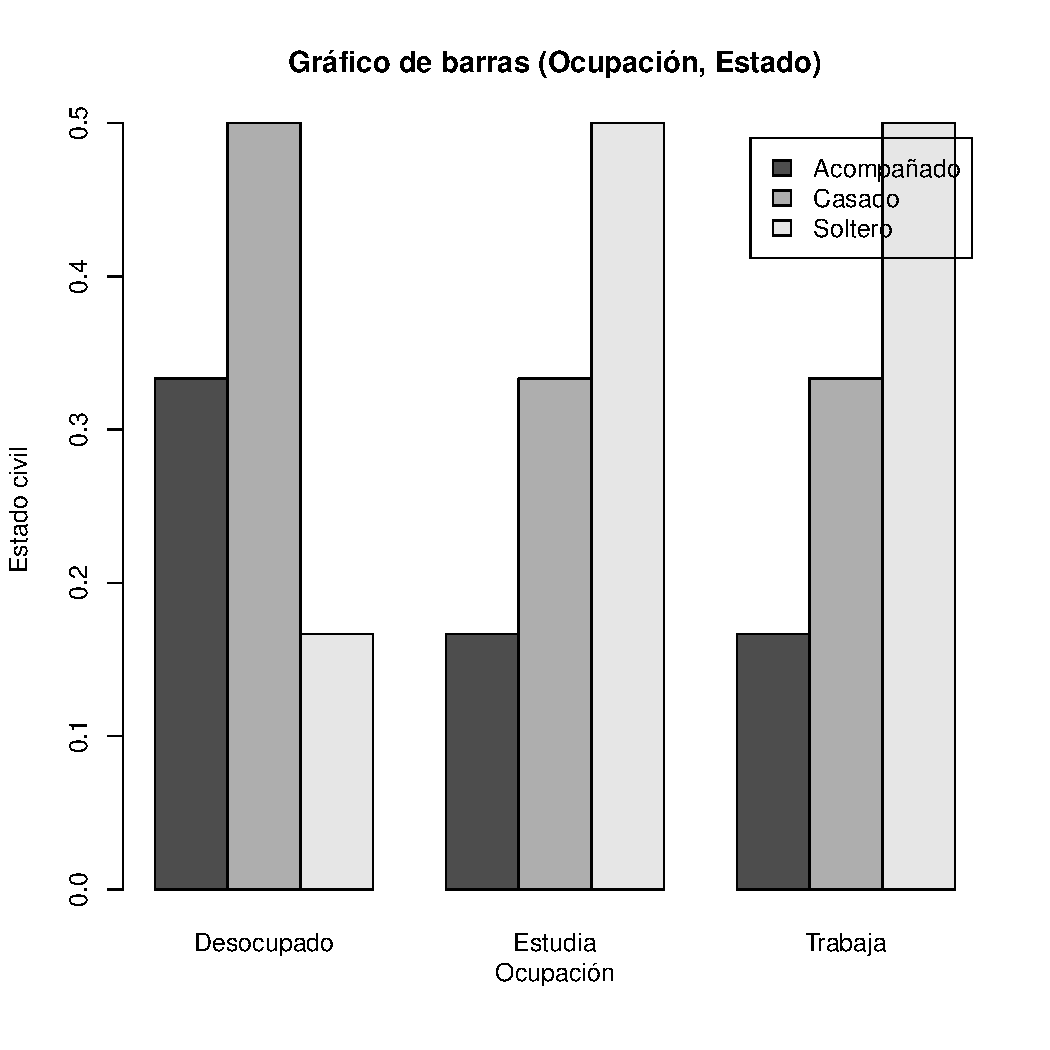
\includegraphics[width=\maxwidth]{figure/unnamed-chunk-1-6} 
\begin{kframe}\begin{alltt}
\hlcom{# Gr�fico de barras no apiladas y colocaci�n de leyenda}
\hlkwd{barplot}\hlstd{(}\hlkwd{table}\hlstd{(Ocupacion, Estado),} \hlkwc{main}\hlstd{=}\hlstr{"Gr�fico de barras (Estado, Ocupaci�n)"}\hlstd{,} \hlkwc{xlab} \hlstd{=}
\hlstr{"Estado civil"}\hlstd{,} \hlkwc{ylab}\hlstd{=}\hlstr{"Ocupaci�n"}\hlstd{,} \hlkwc{beside}\hlstd{=}\hlnum{TRUE}\hlstd{,} \hlkwc{legend.text}\hlstd{=T)}
\end{alltt}
\end{kframe}
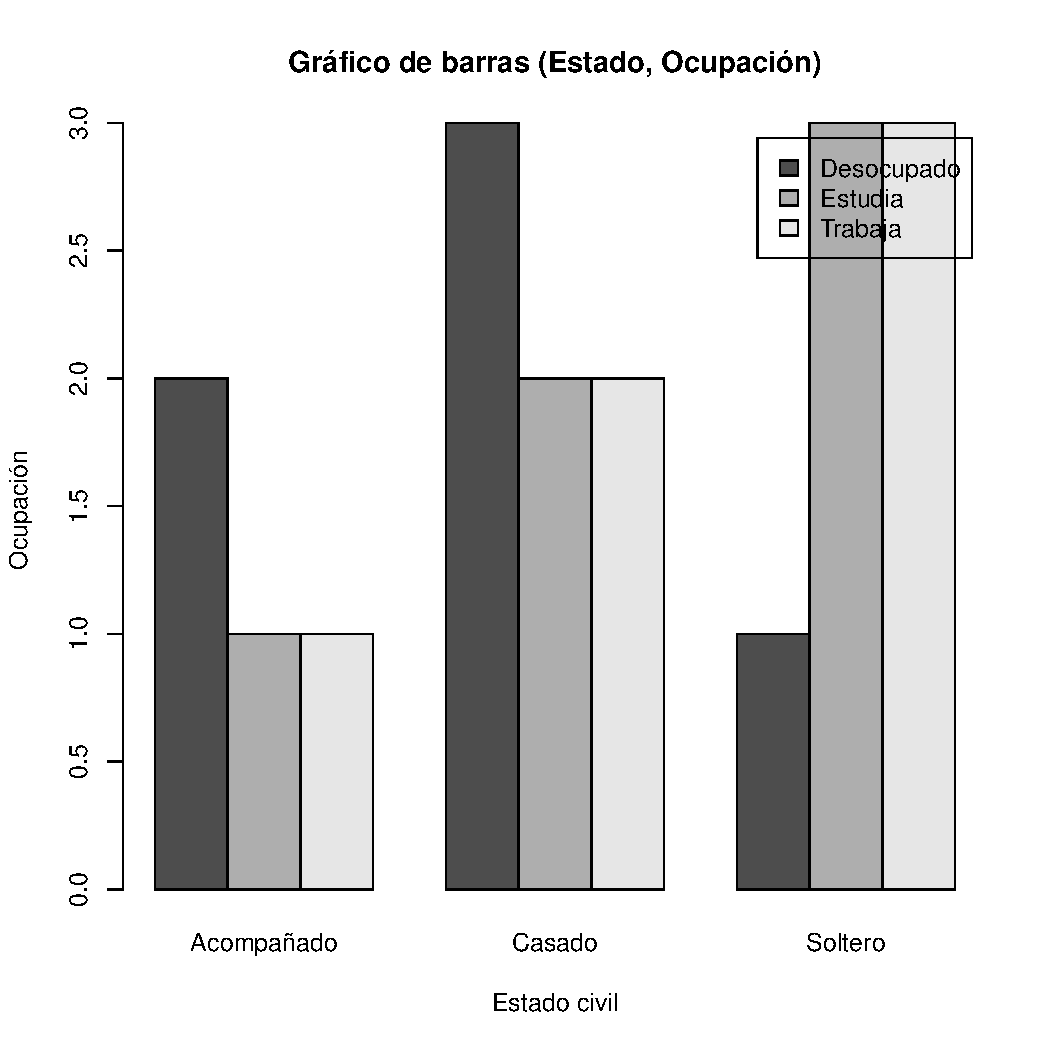
\includegraphics[width=\maxwidth]{figure/unnamed-chunk-1-7} 
\begin{kframe}\begin{alltt}
\hlkwd{barplot}\hlstd{(}\hlkwd{table}\hlstd{(Estado, Ocupacion),} \hlkwc{main}\hlstd{=}\hlstr{"Gr�fico de barras (Ocupaci�n, Estado)"}\hlstd{,} \hlkwc{xlab} \hlstd{=}
\hlstr{"Ocupaci�n"}\hlstd{,} \hlkwc{ylab}\hlstd{=}\hlstr{"Estado civil"}\hlstd{,} \hlkwc{beside}\hlstd{=}\hlnum{TRUE}\hlstd{,} \hlkwc{legend.text}\hlstd{=}\hlnum{TRUE}\hlstd{)}
\end{alltt}
\end{kframe}
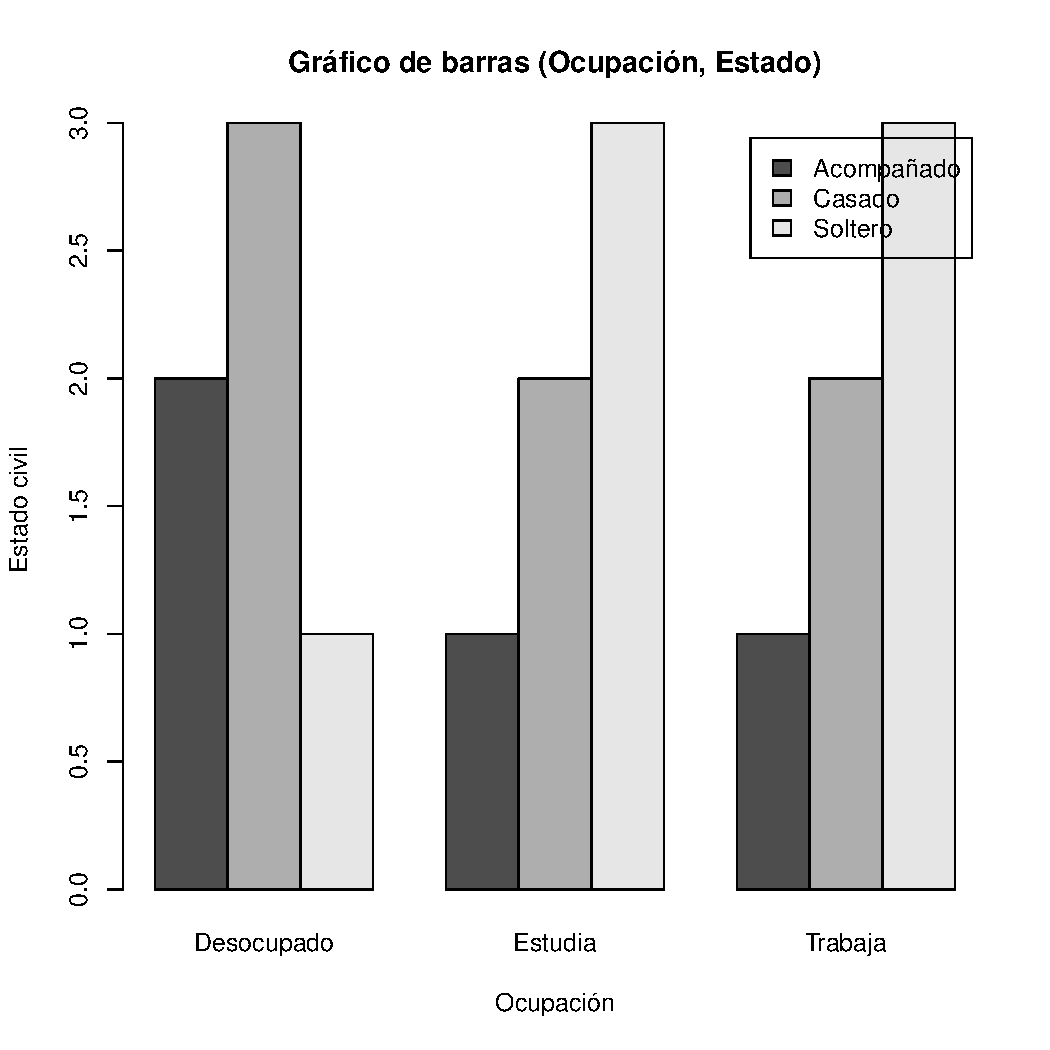
\includegraphics[width=\maxwidth]{figure/unnamed-chunk-1-8} 
\begin{kframe}\begin{alltt}
\hlkwd{barplot}\hlstd{(}\hlkwd{table}\hlstd{(Estado, Ocupacion),} \hlkwc{main}\hlstd{=}\hlstr{"Gr�fico de barras (Ocupaci�n, Estado)"}\hlstd{,}
\hlkwc{xlab}\hlstd{=}\hlstr{"Ocupaci�n"}\hlstd{,} \hlkwc{ylab}\hlstd{=}\hlstr{"Estado civil"}\hlstd{,} \hlkwc{beside}\hlstd{=}\hlnum{TRUE}\hlstd{,} \hlkwc{legend.text}\hlstd{=}\hlkwd{c}\hlstd{(}\hlstr{"menor que 2"}\hlstd{,} \hlstr{"2-3"}\hlstd{,}
\hlstr{"mayor que 3"}\hlstd{))}
\end{alltt}
\end{kframe}
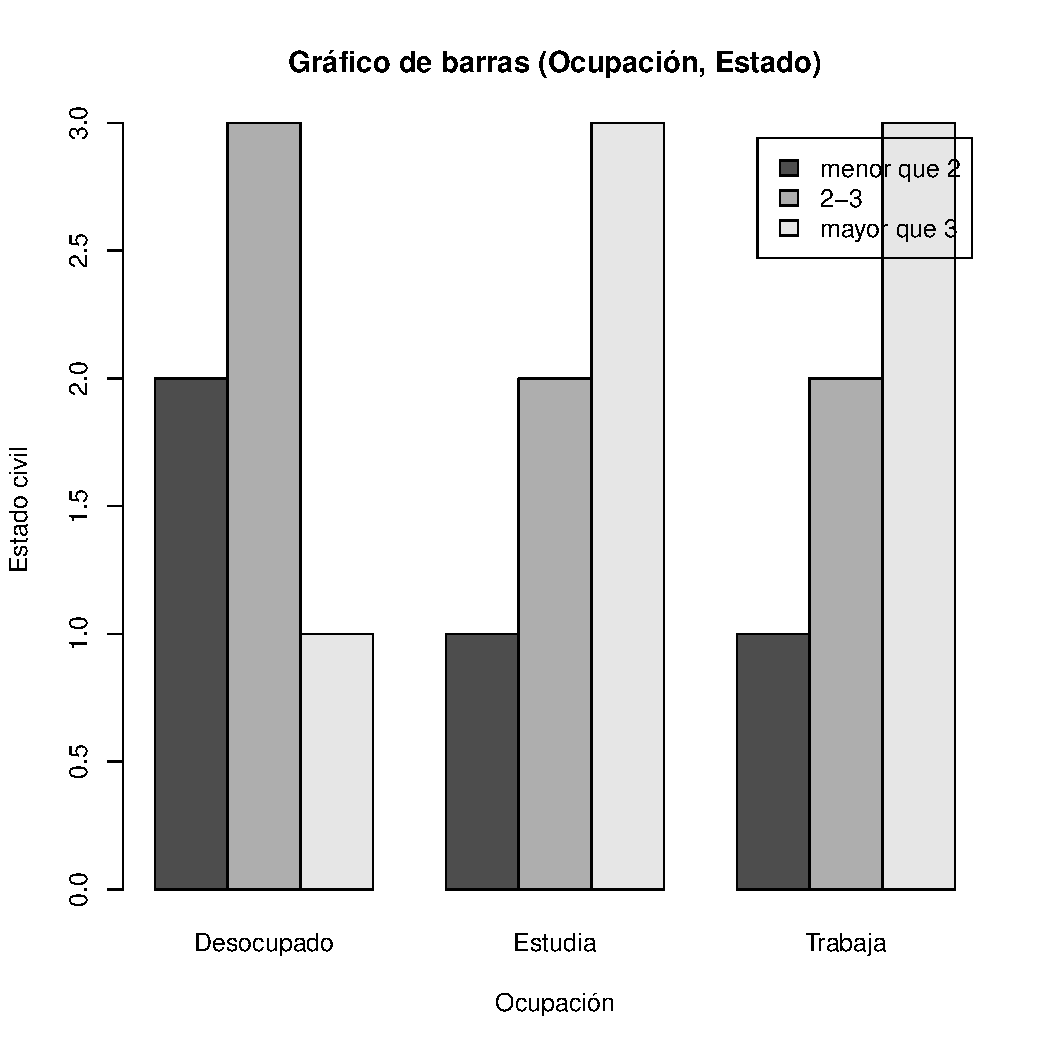
\includegraphics[width=\maxwidth]{figure/unnamed-chunk-1-9} 
\begin{kframe}\begin{alltt}
\hlcom{#Realizar la prueba o contraste Chi-cuadrado de independencia}
\hlstd{prueba} \hlkwb{<-} \hlkwd{chisq.test}\hlstd{(tablaCont); prueba}
\end{alltt}


{\ttfamily\noindent\color{warningcolor}{\#\# Warning in chisq.test(tablaCont): Chi-squared approximation may be incorrect}}\begin{verbatim}
## 
## 	Pearson's Chi-squared test
## 
## data:  tablaCont
## X-squared = 2, df = 4, p-value = 0.7
\end{verbatim}
\begin{alltt}
\hlcom{# Frecuencias absolutas esperadas para la prueba Chi-cuadrada}
\hlstd{prueba}\hlopt{$}\hlstd{expected} \hlcom{# fij = fi./No. column}
\end{alltt}
\begin{verbatim}
##             Ocupacion
## Estado       Desocupado Estudia Trabaja
##   Acompa�ado       1.33    1.33    1.33
##   Casado           2.33    2.33    2.33
##   Soltero          2.33    2.33    2.33
\end{verbatim}
\end{kframe}
\end{knitrout}
\end{document}
